\documentclass[11pt]{article}

\usepackage[margin=0.75in]{geometry}
\usepackage{graphicx}
\usepackage{booktabs}
\usepackage{float}
\usepackage{hyperref}
\usepackage{xcolor}
\usepackage{array}

\hypersetup{
  colorlinks=true,
  linkcolor=blue!55!black,
  urlcolor=blue!55!black,
  citecolor=blue!55!black
}

\title{Yichao Brightfield-to-Fluorescence Pix2Pix Result Report}
\author{OrganoidAgent}
\date{May 11, 2026}

\begin{document}
\maketitle

\section*{Summary}

This report documents the corrected same-time brightfield-to-fluorescence (B2F) experiment for the Yichao projected organoid instance dataset. The goal is to establish whether the paired brightfield crop contains enough morphological information to reconstruct or classify fluorescence before using the model for future-expression prediction.

The successful run used the older pix2pix-style U-Net family that previously worked well in \path{/home/lachlan/ProjectsLFS/OrganoidAgent/pixel2pixel_fluorescent/fluorescent/cyclegan_modules.py}, adapted to the projected instance-pair database. Training used original 384 pixel crops, no AMP, balanced sampling, and resumable early stopping. The run stopped at epoch 78 after validation convergence was detected; the best validation checkpoint was epoch 10.

\section*{Data and Model}

The training data came from the projected instance-pair manifest:
\[
\mathcal{D}=\{(B_i,F_i,M_i)\}_{i=1}^N,
\]
where \(B_i\) is the brightfield crop, \(F_i\) is the corresponding fluorescence crop, and \(M_i\) is the organoid mask. The split sizes were 6691 training instances, 1601 validation instances, and 1088 held-out test instances.

The model was a pix2pix-style U-Net with InstanceNorm and ELU blocks. For each brightfield image, the network predicts fluorescence logits:
\[
\hat F_i=\sigma(G_\theta(B_i)).
\]
The objective combined weighted fluorescence reconstruction, pixel BCE, structure, edge, and scalar auxiliary terms. Bright fluorescence pixels received higher weight so the sparse signal was not overwhelmed by dark background.

\section*{Training and Early Stopping}

The early-stop score was reconstruction-first:
\[
s = -\mathcal{L}_{val} + 0.05\,\mathrm{F1}_{signal} + 0.01\,r_{peak}.
\]
Training stopped when this score failed to improve by at least 0.001 for 10 validation checks after epoch 40. On resume, the trainer scanned the existing metrics and detected that the model had already converged.

\begin{figure}[H]
  \centering
  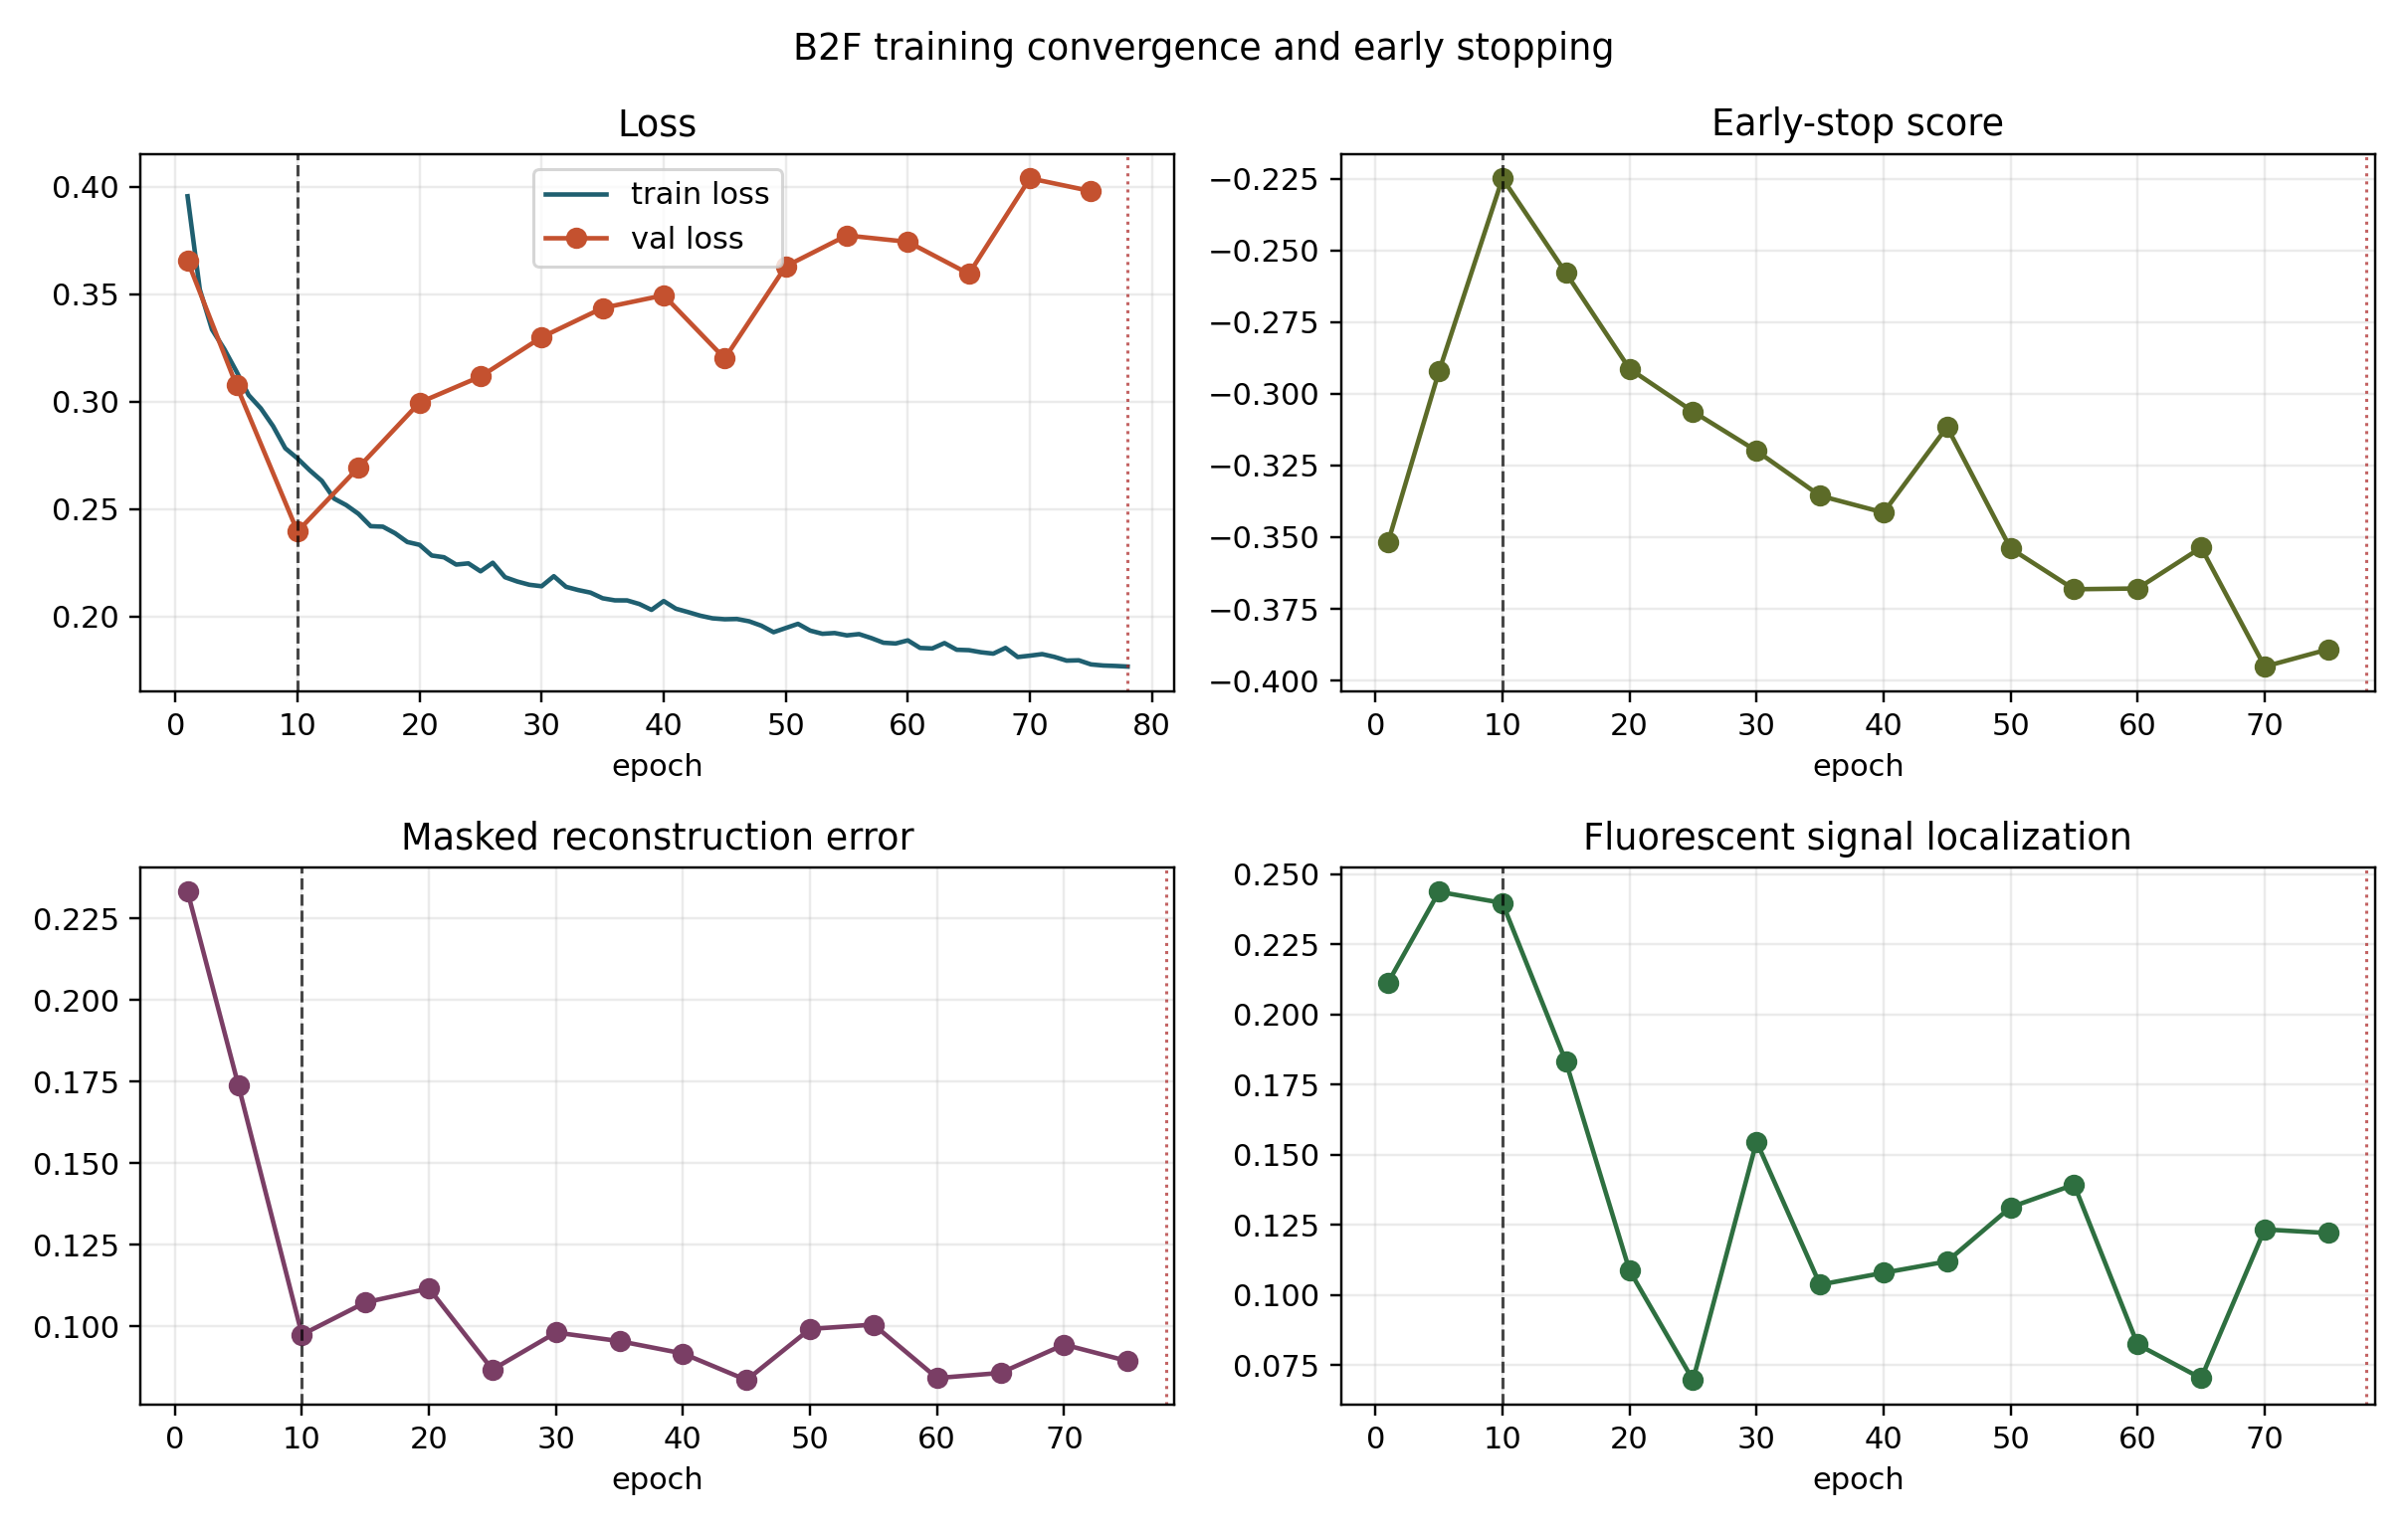
\includegraphics[width=\textwidth]{figures/fig1_training_convergence.png}
  \caption{Training convergence, validation loss, early-stop score, masked MAE, and fluorescent signal F1. The best checkpoint occurred early, while later epochs continued improving training loss but degraded validation score.}
\end{figure}

\section*{Held-Out Quantification}

\begin{table}[H]
  \centering
  \caption{Main held-out test metrics from the best checkpoint.}
  \begin{tabular}{ll}
\toprule
Quantity & Value \\
\midrule
Best epoch & 10 \\
Stop epoch & 78 \\
Test signal F1 & 0.387 \\
Test signal precision & 0.266 \\
Test signal recall & 0.710 \\
Test expression AUROC & 0.879 \\
Test masked MAE & 0.096 \\
Test PSNR & 18.03 dB \\
\bottomrule
\end{tabular}

\end{table}

\begin{figure}[H]
  \centering
  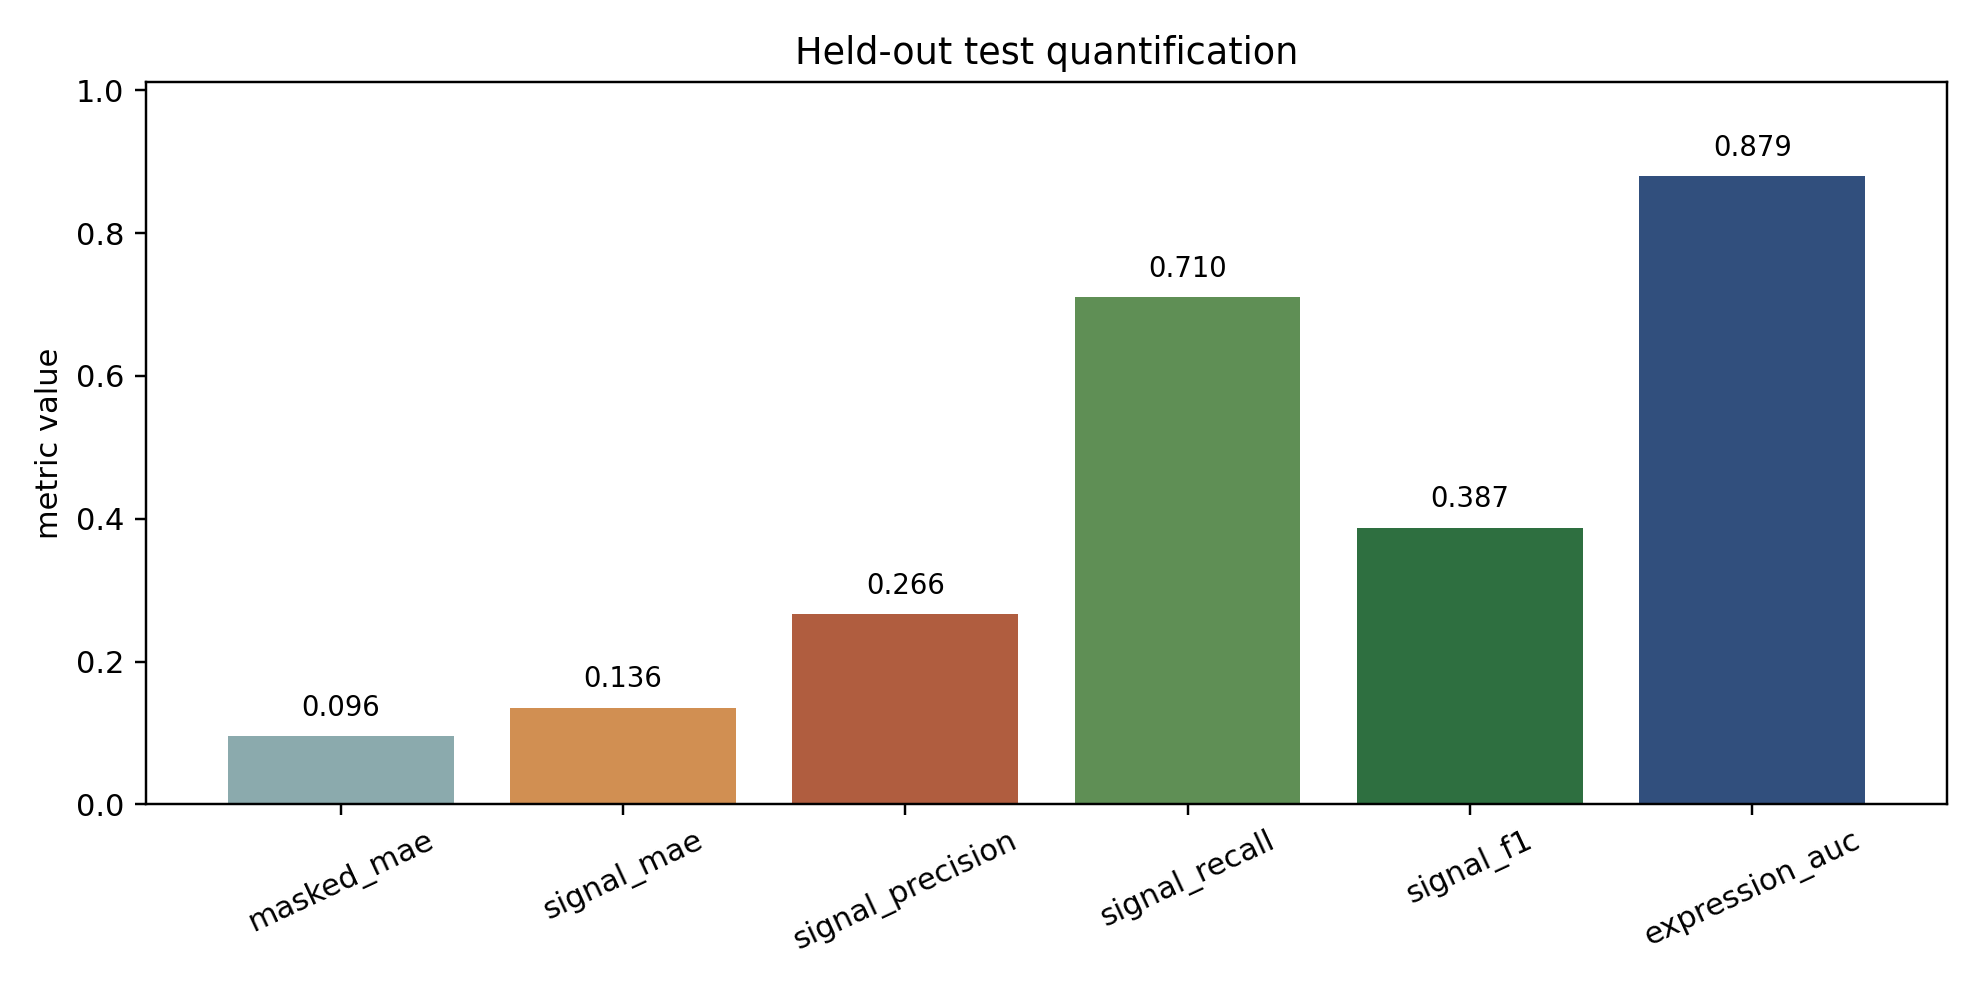
\includegraphics[width=0.88\textwidth]{figures/fig2_test_quantification.png}
  \caption{Aggregate test-set metrics. The model has high recall and moderate precision, consistent with a useful but over-inclusive fluorescence predictor.}
\end{figure}

\begin{table}[H]
  \centering
  \caption{Per-dataset held-out test summary. True and predicted signal values are fractions of masked organoid pixels above the fluorescence threshold.}
  \resizebox{\textwidth}{!}{\begin{tabular}{lrrrrr}
\toprule
Dataset & $n$ & True signal & Pred signal & Signal F1 & Masked MAE \\
\midrule
Data-Yichao-1 & 1 & 0.000 & 0.165 & 0.003 & 0.145 \\
Data-Yichao-2 & 33 & 0.154 & 0.124 & 0.178 & 0.122 \\
Data-Yichao-3 & 345 & 0.053 & 0.290 & 0.130 & 0.117 \\
Data-Yichao-5 & 180 & 0.002 & 0.103 & 0.007 & 0.099 \\
Data-Yichao-6 & 86 & 0.018 & 0.087 & 0.039 & 0.078 \\
Data-Yichao-7 & 170 & 0.024 & 0.053 & 0.064 & 0.060 \\
Data-Yichao-9 & 273 & 0.370 & 0.745 & 0.501 & 0.098 \\
\bottomrule
\end{tabular}
}
\end{table}

\begin{figure}[H]
  \centering
  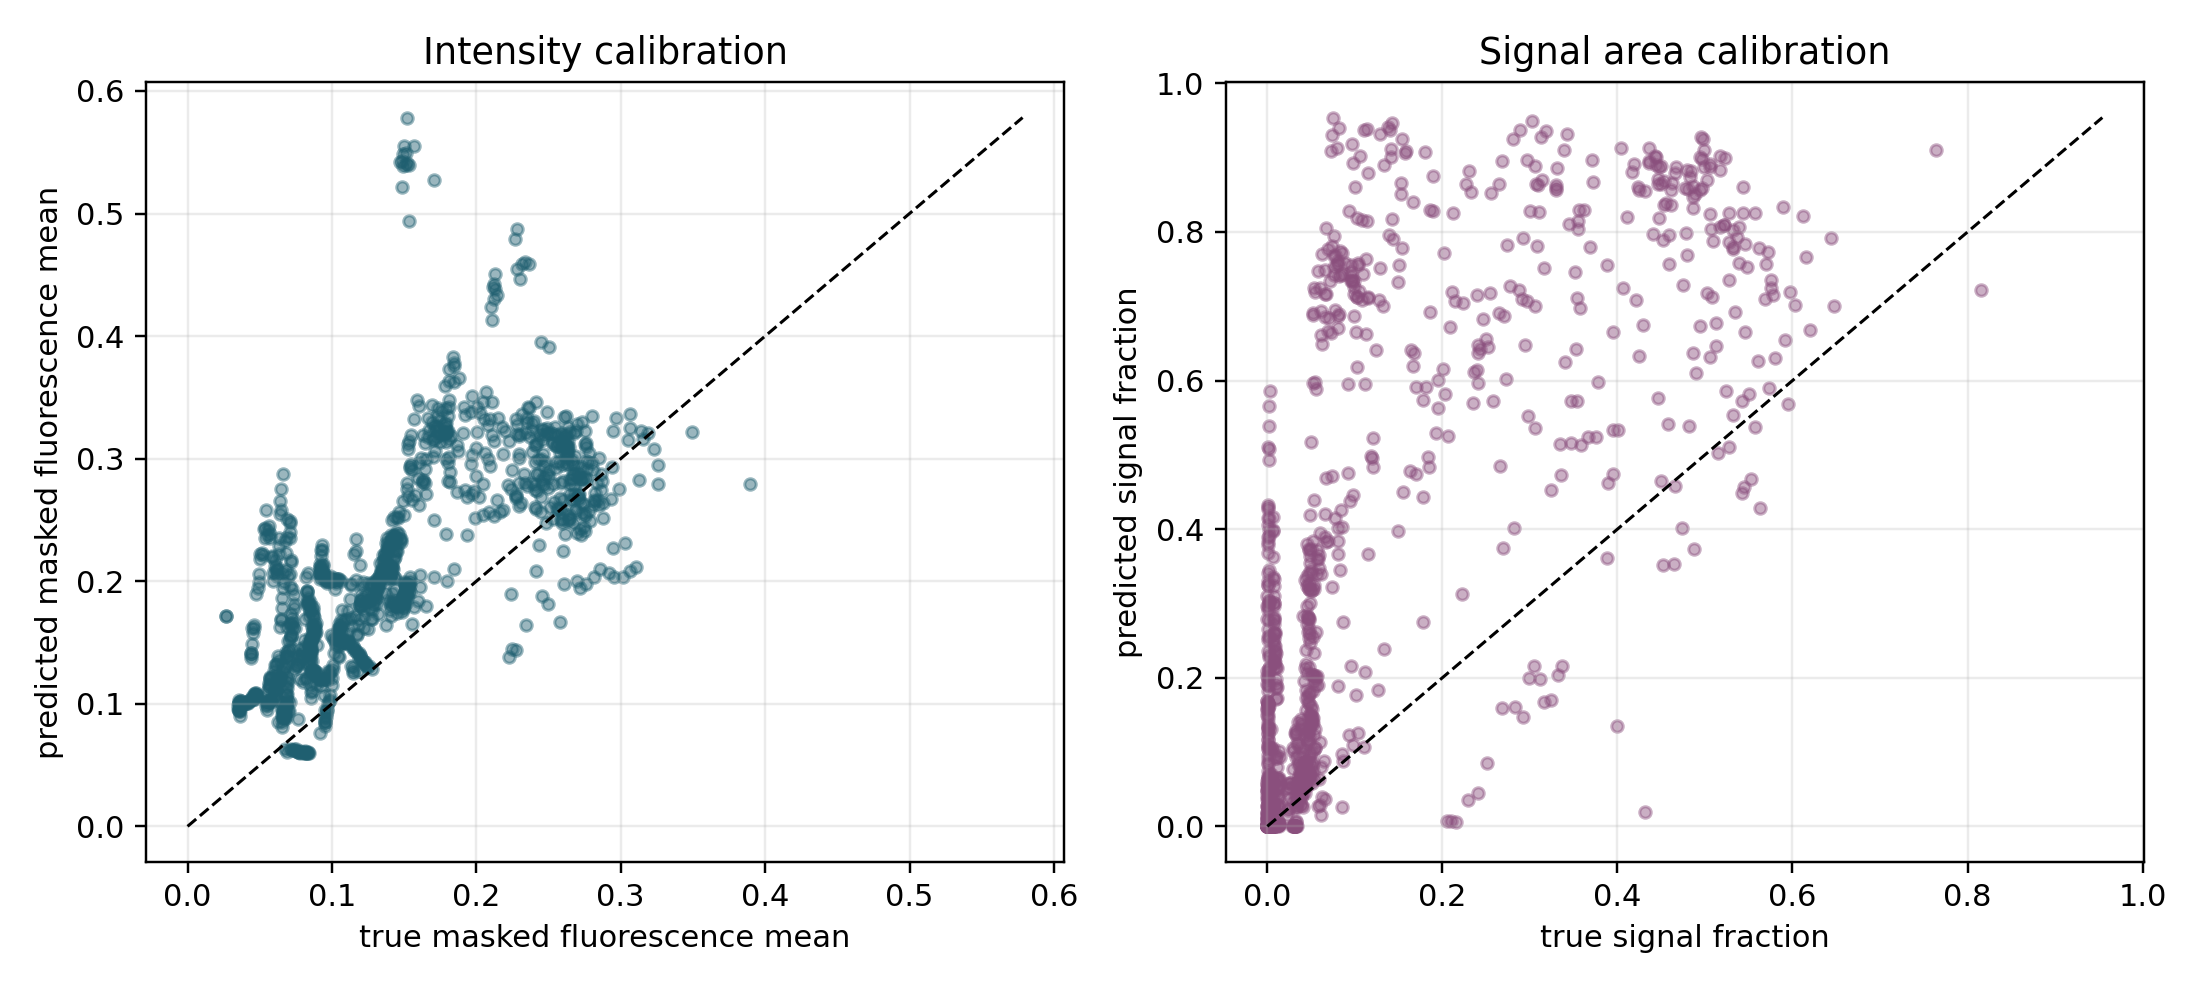
\includegraphics[width=\textwidth]{figures/fig4_prediction_calibration.png}
  \caption{Per-instance calibration on the held-out test set. Left: masked mean fluorescence. Right: fluorescent signal area. The masked mean correlation was 0.692, but signal area tends to be over-predicted for weak or negative examples.}
\end{figure}

\section*{Prediction Visualizations}

\begin{figure}[H]
  \centering
  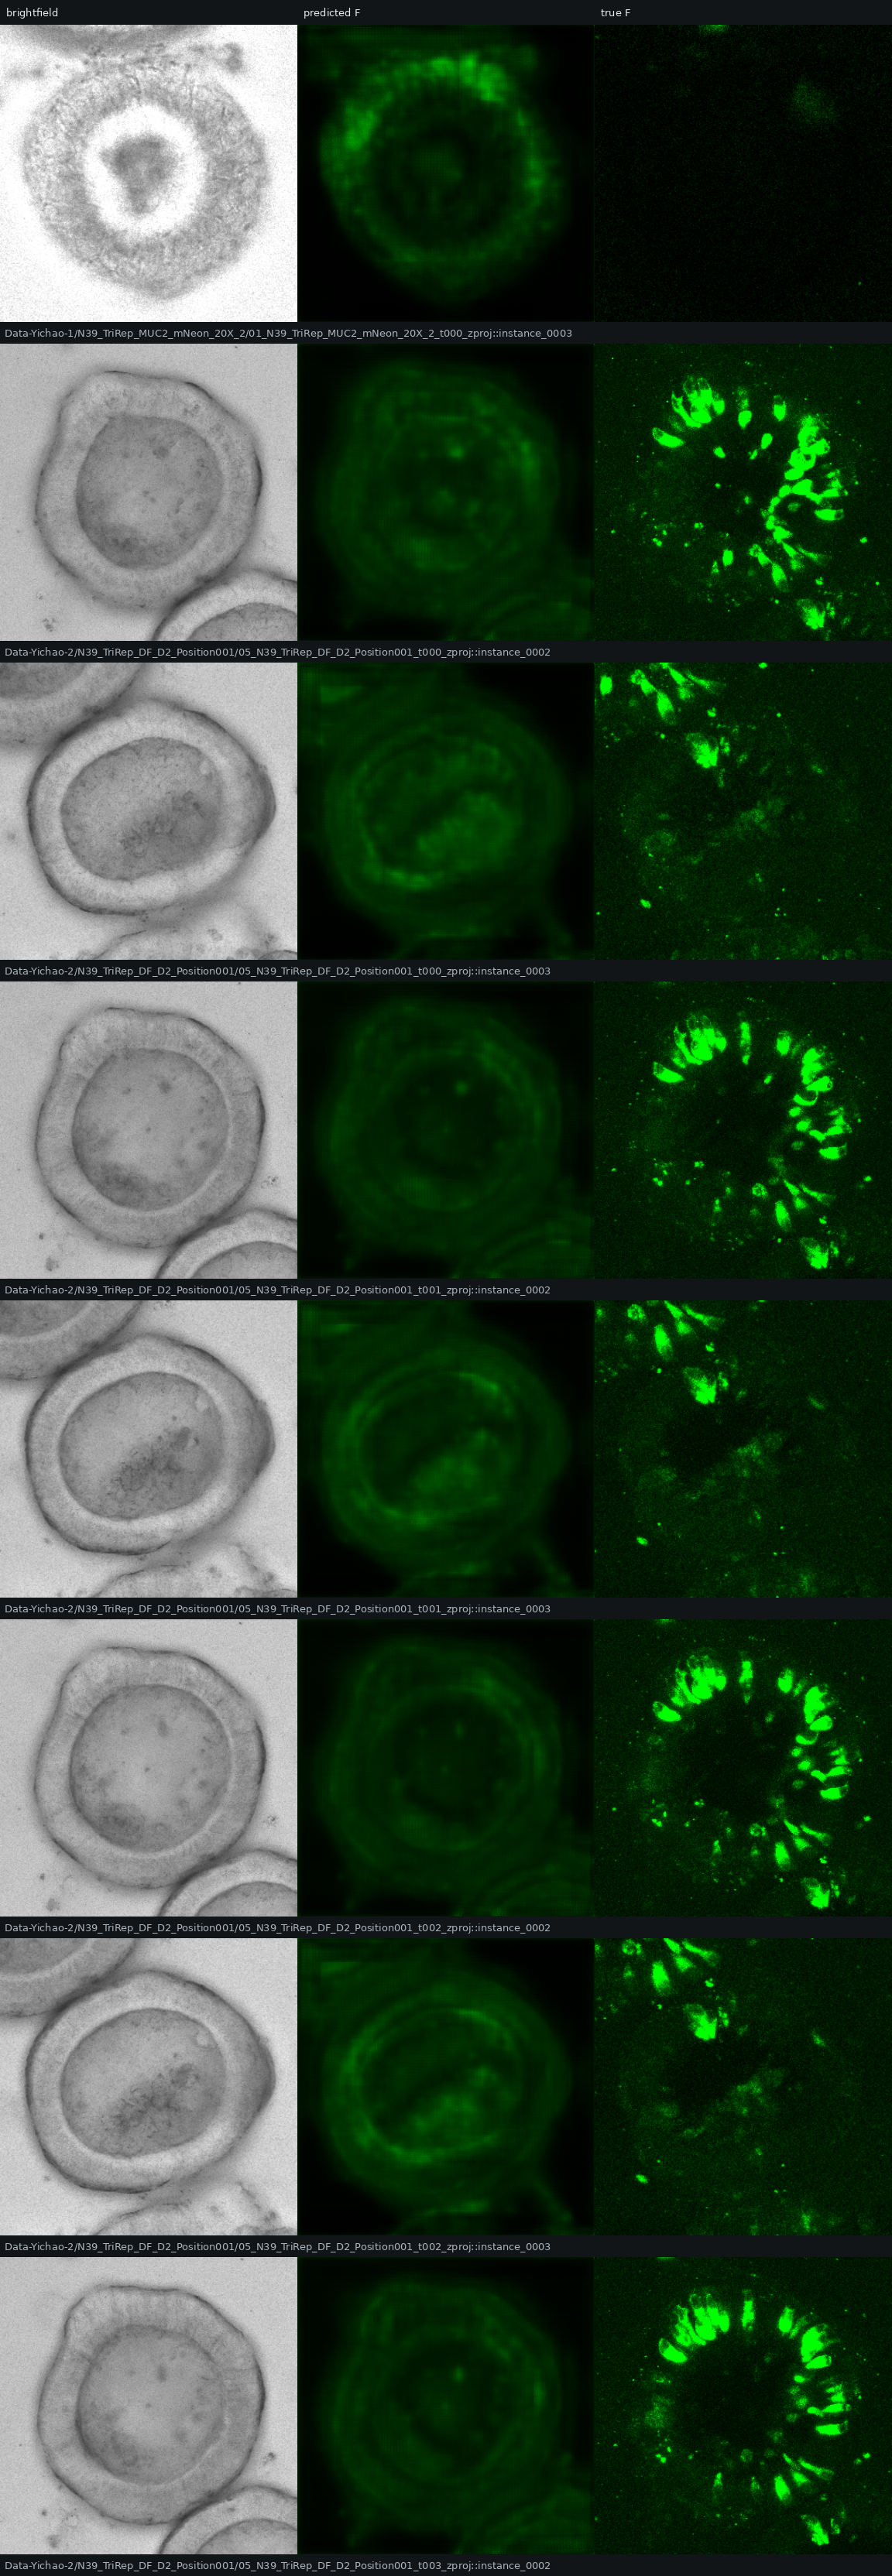
\includegraphics[height=0.82\textheight]{figures/fig3_test_best_panel.png}
  \caption{Original held-out test panel saved by the trainer: brightfield input, predicted fluorescence, and true fluorescence.}
\end{figure}

\begin{figure}[H]
  \centering
  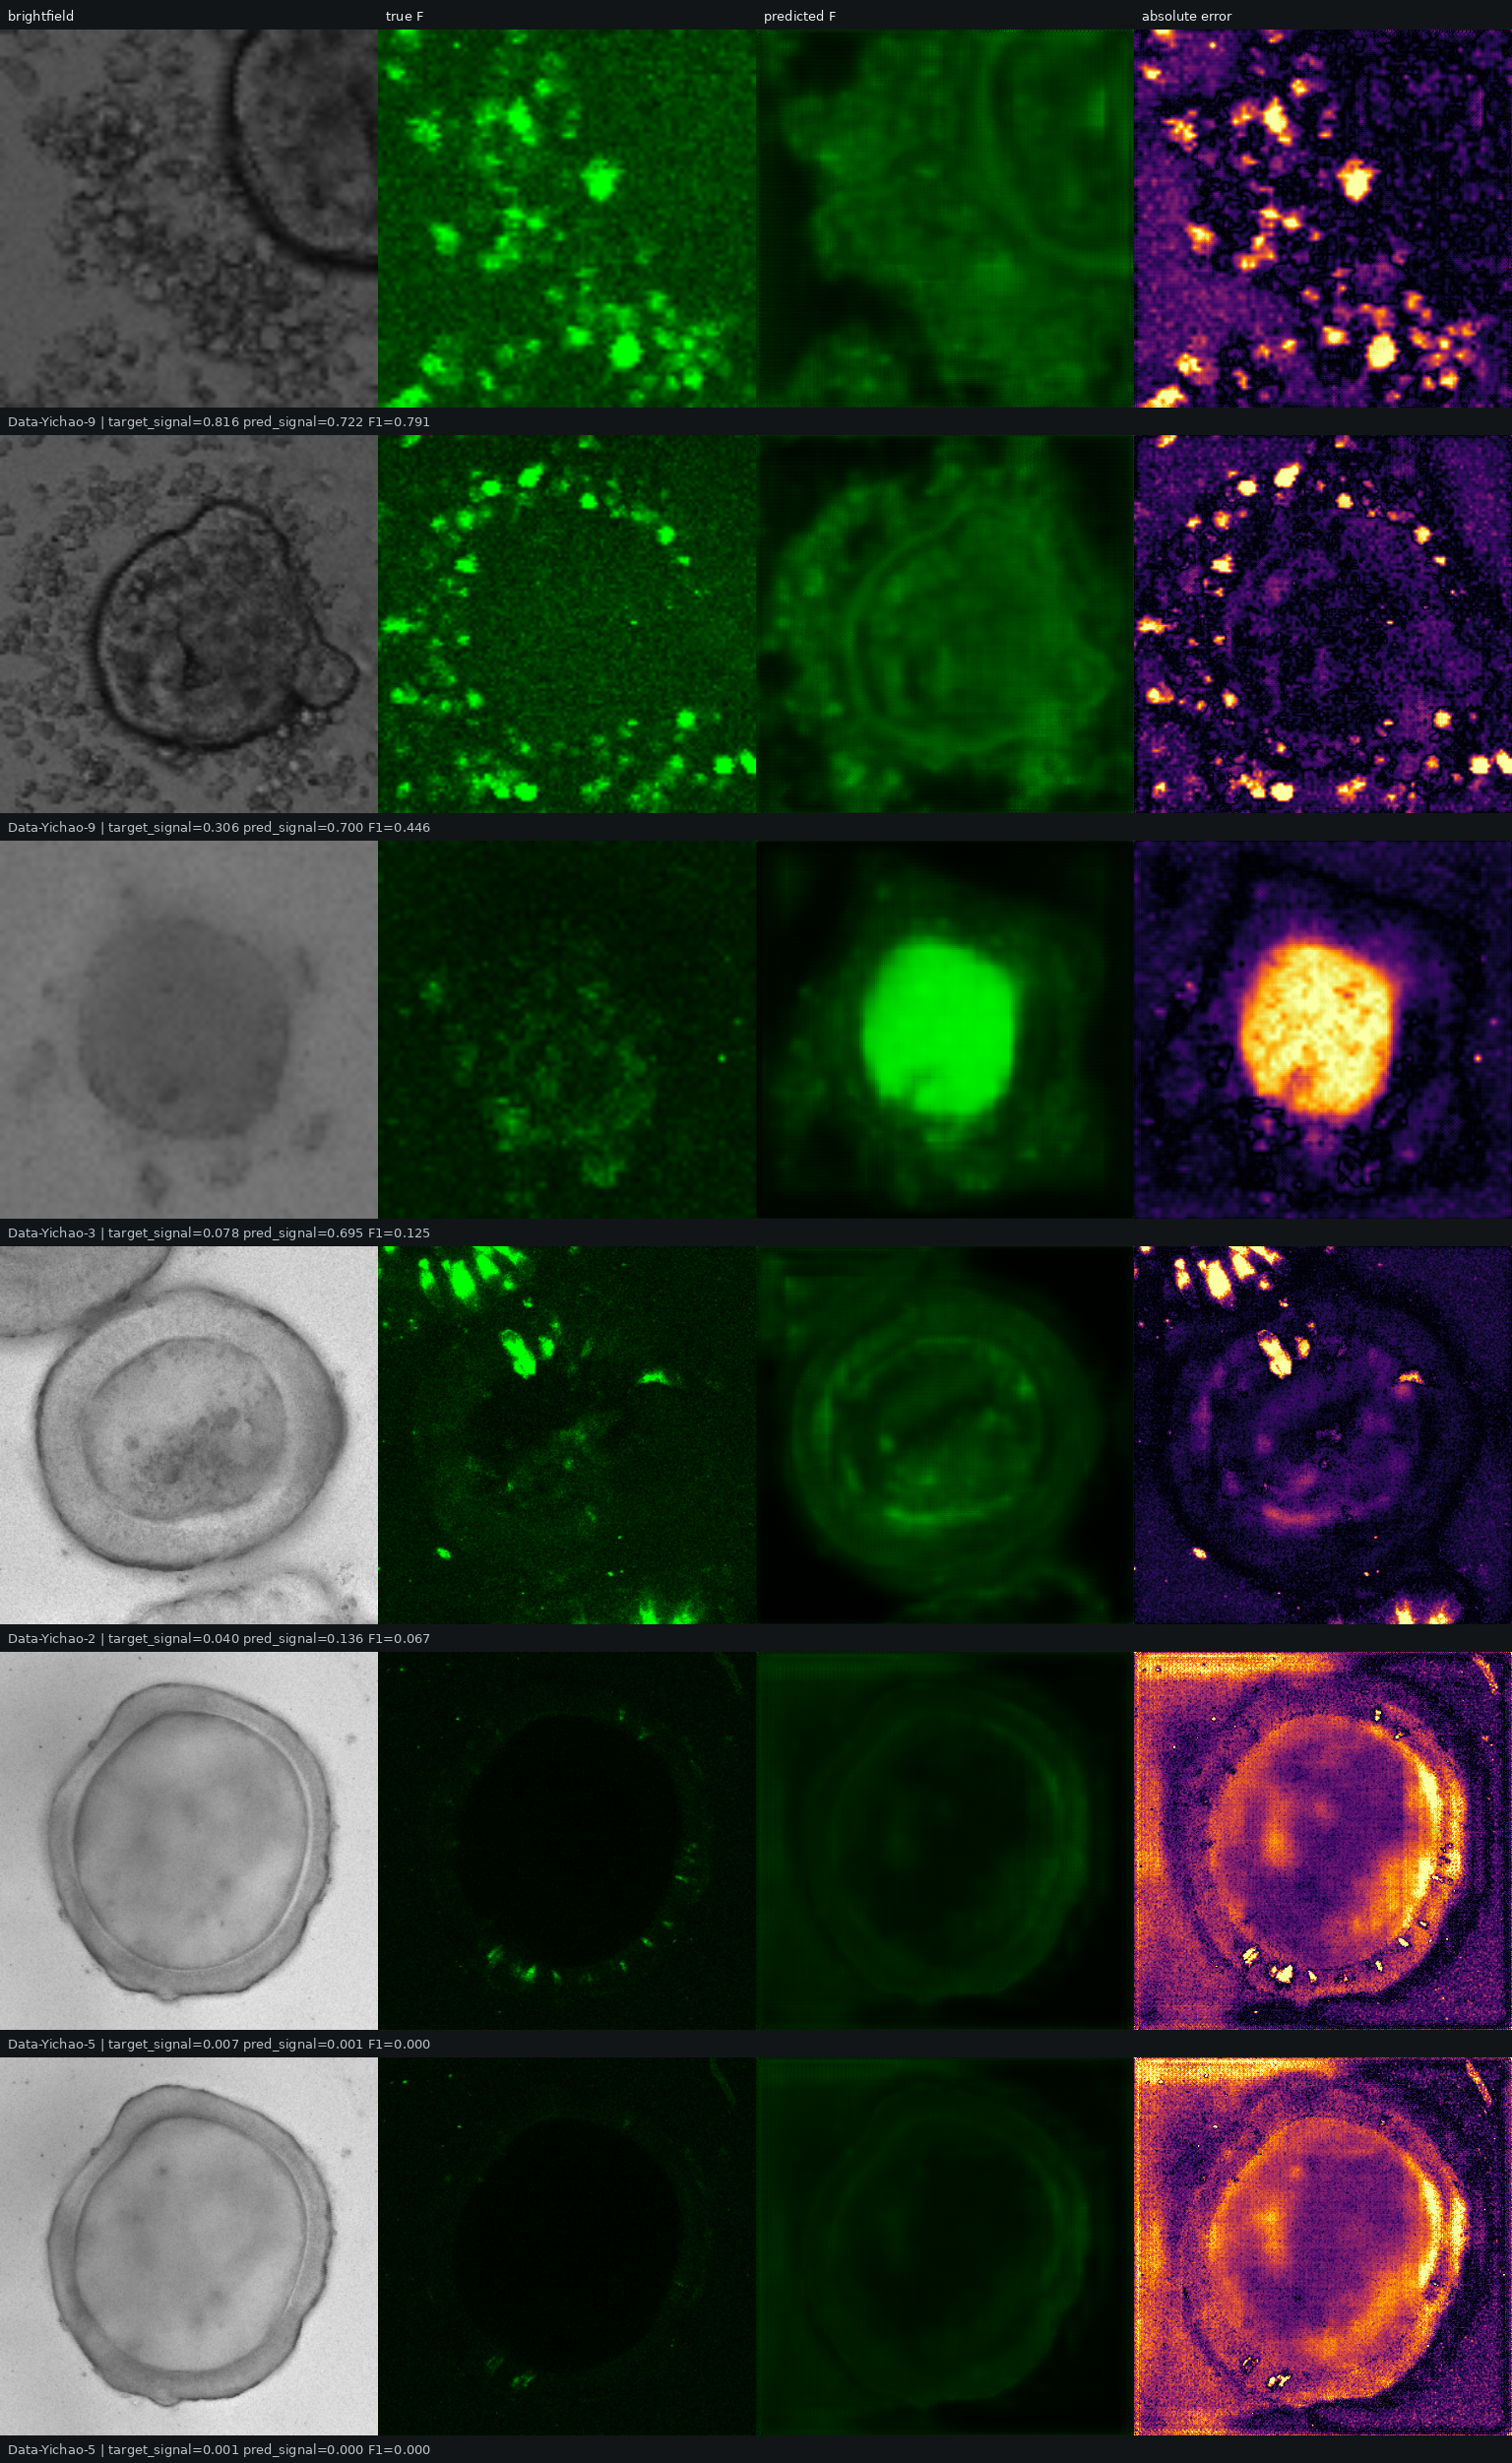
\includegraphics[height=0.82\textheight]{figures/fig5_prediction_error_examples.png}
  \caption{Selected held-out examples with brightfield input, true fluorescence, predicted fluorescence, and absolute error. The model often captures broad positive regions, but can over-predict signal in low-expression cases.}
\end{figure}

\section*{Explanation}

The explanation figure uses input-gradient saliency. For each selected held-out crop, the objective was the mean predicted fluorescence inside the organoid mask:
\[
a(B)=\frac{1}{|M|}\sum_{x\in M}\hat F(x),
\quad
S(x)=\left|\frac{\partial a}{\partial B(x)}\right|.
\]
This is a model-sensitivity map, not a causal biological proof. It indicates which brightfield pixels the trained B2F model most relied on when increasing predicted fluorescence.

\begin{figure}[H]
  \centering
  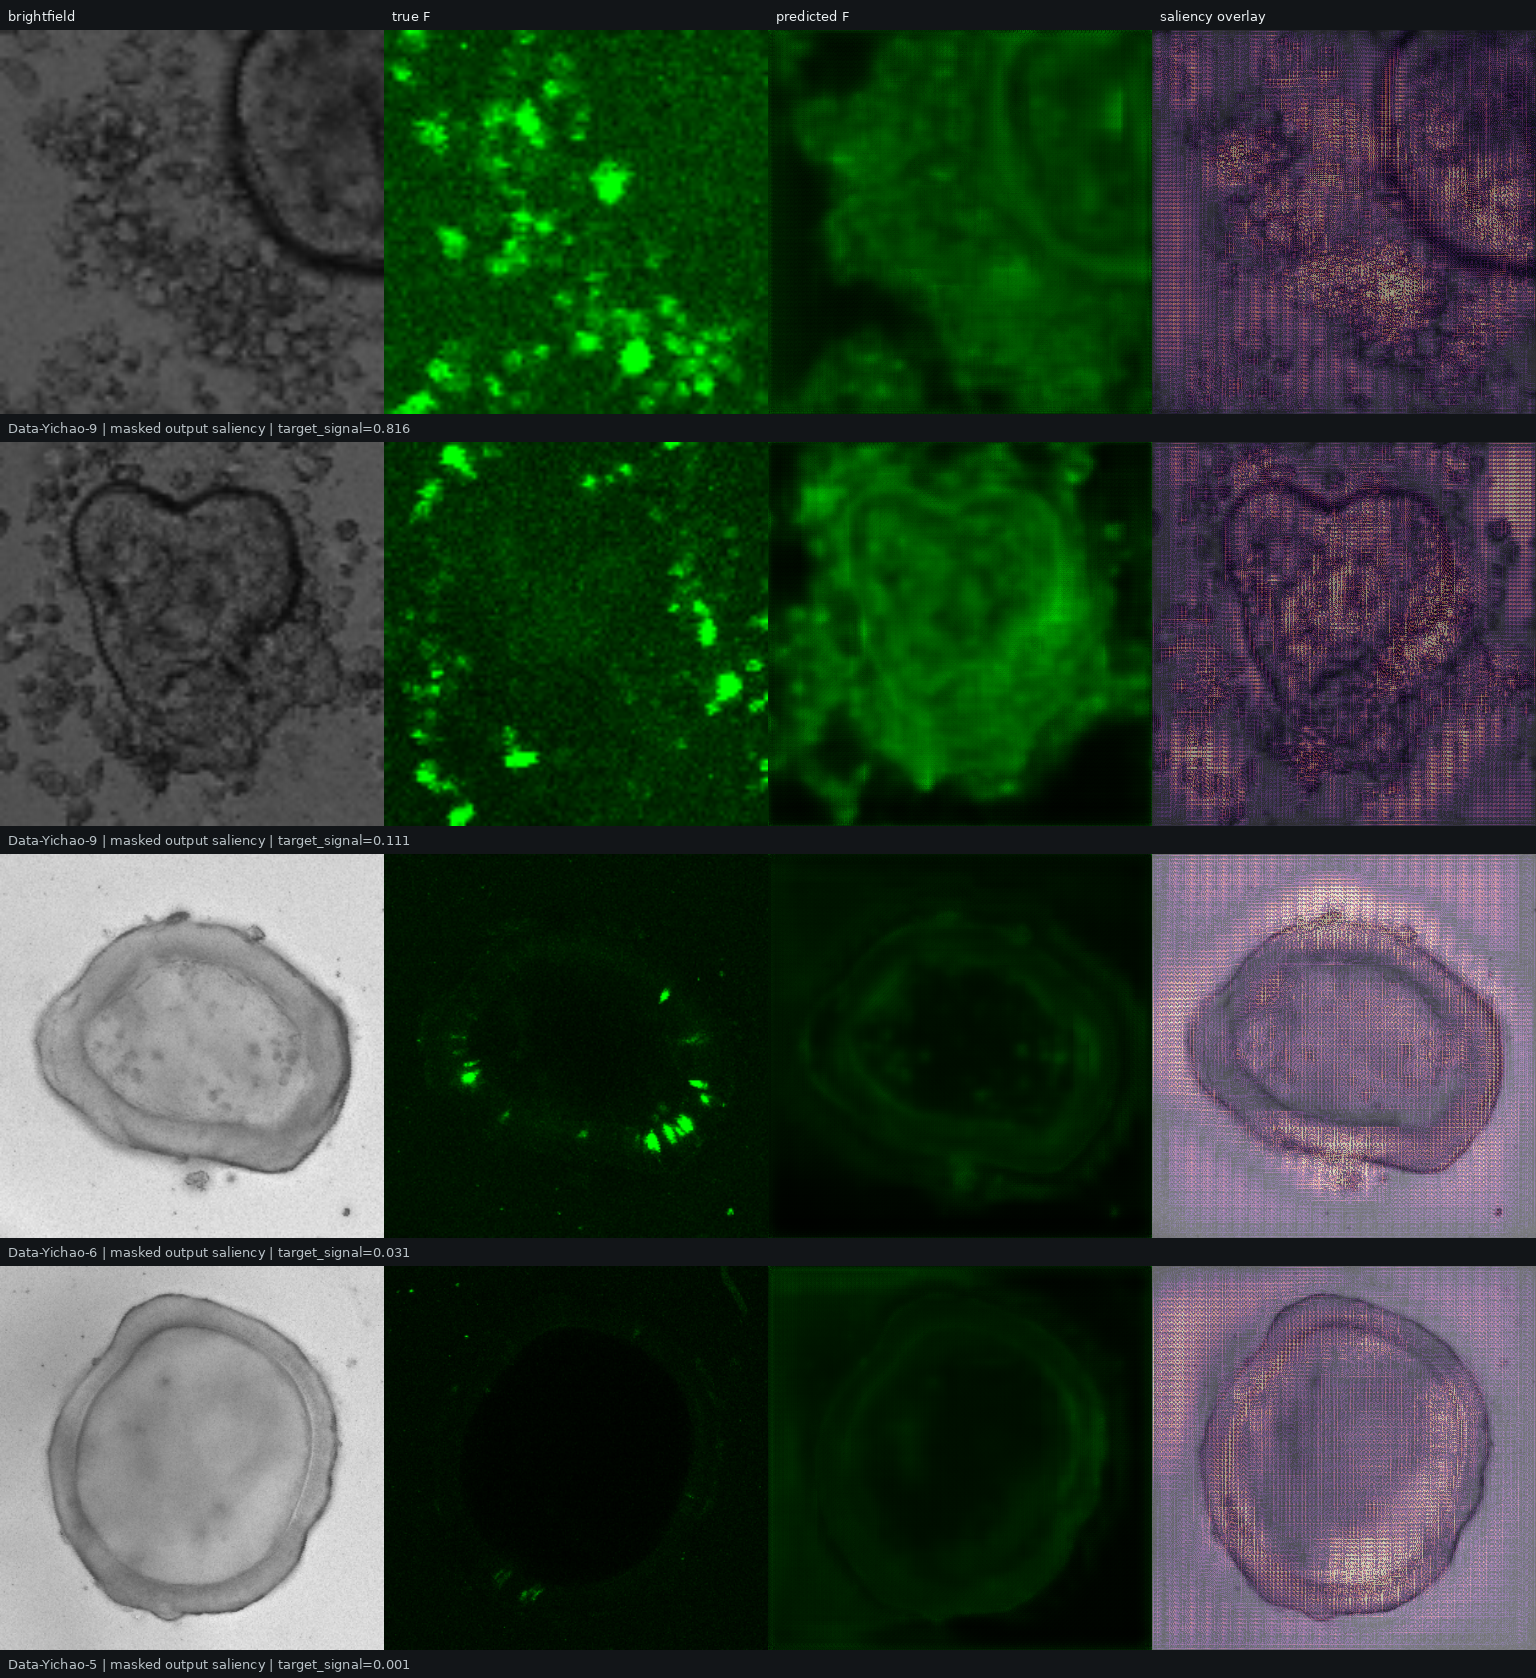
\includegraphics[width=\textwidth]{figures/fig6_saliency_explanation.png}
  \caption{Gradient saliency overlays. The highlighted regions tend to follow organoid texture and boundary structure, supporting the interpretation that the model is using morphology rather than a constant intensity prior.}
\end{figure}

\section*{Interpretation}

The corrected B2F experiment is now technically valid: optimizer steps occurred, validation was monitored, and early stopping selected the best checkpoint. The held-out test AUROC for expression classification was 0.879, indicating that brightfield morphology contains information associated with fluorescence-positive status.

The reconstruction is not yet perfect. Signal recall was 0.710, but precision was 0.266, so the model tends to predict too much fluorescent area. The per-dataset table shows that performance is strongest on Data-Yichao-9, while low-expression datasets expose over-prediction. This matters for the next phase: future-expression prediction should not use raw predicted pixel area alone. It should combine calibrated B2F outputs with morphology, time, position, and expression onset analysis.

\section*{Artifacts}

The artifact generator is:
\begin{center}
\small\path{/home/lachlan/ProjectsLFS/OrganoidAgent/differentiation_prediction/yichao_future_expression/make_b2f_result_artifacts.py}
\end{center}

The finished run is:
\begin{center}
\small\path{/home/lachlan/ProjectsLFS/OrganoidAgent/analysis-outputs/yichao_future_expression/stage1_b2f_pix2pix_384_v1_noamp_long}
\end{center}

The generated per-instance test quantification table is:
\begin{center}
\small\path{/home/lachlan/ProjectsLFS/OrganoidAgent/publication/yichao_b2f_pix2pix_results_report/tables/test_per_instance_quantification.csv}
\end{center}

\end{document}
